\section{Durchführung}
\label{sec:Durchführung}
Der Versuch wird, wie in Abbildung \ref{fig:aufb} zu sehen, aufgebaut.
\begin{figure}
    \centering
    \caption{Versuchsaufbau \cite{V400}}
    \label{fig:aufb}
    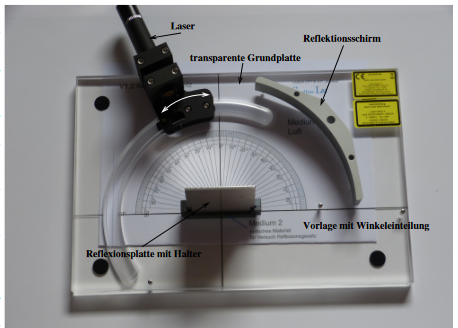
\includegraphics[width = 0.6 \textwidth]{pics/aufb.png}
\end{figure}
Dabei wird die Reflexionsplatte je nach Aufgabenstellung ausgetauscht.
Die wichtigsten Teile des Aufbaus ist eine transparente Grundplatte auf der sich zwei Laserdiodenmodule befinden, die sich im Halbkreis bewegen lassen.
Dabei emittiert die obere Laserdiode rotes Licht der Wellenlänge $\lambda = \SI{635}{\nano \meter}$ und die untere grünes Licht der Wellenlänge $\lambda=\SI{532}{\nano \meter}$.
Bei allen Experimenten ist das optisch dünnere Medium Luft mit der Lichtgeschwindigkeit $c$ und dem Brechungsindex $n \approx 1$.\\
Ein Reflexionsschirm befindet sich am Ende des Hlabkreises zum Schutz vor dem Laserlicht. Die Winkel können mit Hilfe des Transmissionsschirmes und verschiedenen Versuchsvorlagen gemessen werden.
Die Versuchsvorlagen werden dabei unter die transparente Platte geschoben.\\
Im ersten Aufgabenteil wird das Reflexionsgesetz überprüft. Verwendet wird hier grünes Licht, eine Spiegelplatte und die Vorlage A.
Der Aufbau ist in Abbildung \ref{fig:aufb} gezeigt. Es werden sieben Ein- und Reflexionswinkel an dem Transmissionsschirm abgelesen, indem die Laserdiode auf dem Halbkreis verschoben wird.
Für den zweiten Versuchsteil wird der Spiegel durch eine planparallele Platte der dicke $d=SI{5.85}{\centi \metre} $ ersetzt. Für das Brechungsgesetz gilt mit $n_1=1$ für Luft die vereinfachte Form
\begin{equation}
    \frac{\sin \alpha}{\sin \beta} = n
\end{equation}
mit $n_2=n$. Es werden erneut sieben Messungen der Ein- und Transmissionswinkel vergenommen. Die Transmissionswinkel können an der auf der planparallelen Platte aufgeklebten Platte abgelesen werde.
Daraus soll sowohl der Brechungsindex $n$ der planparallelen Platte, als auch der Strahlversatz ermittelt werden.
Der Strahlversatz lässt sich mit
\begin{equation}
    s=d \frac{\sin\left(\alpha- \beta\right)}{\cos \beta}
    \label{eqn:strahlversatz}
\end{equation}
berechnen. 
Im nächsten Teil wird die planparallele Platte mit einem Prisma ersetzt. Es wird das grüne und rote Licht verwendet um die Ablenkungen im Prisma zu untersichen. Dabei lässt sich
die Ablenkung durch
\begin{equation}
    \delta= (\alpha_1 + \alpha_2)- (\beta_1+ \beta_2)
    \label{eqn:ablenk}
\end{equation}
berechnen. Der Winkel $\alpha_1$ ist dabei der Einfallswinkel und $\alpha_2$ ist der Austrittswinkel. Die Winkel $\beta_k$ sind dabei die Winkel im inneren des Prismas, sie können mit Hilfe des Brechungsgesetzes berechnet werden
Für beide Laser werden fünf verschiedene Ein- und Ausfallswinkel gemessen. 
Im letzen Versuchsteil wird die Beugung am Gitter untersucht. Das Gitter wird an das eine Ende der transparenten Platte positioniert und die Laser werden Senkrecht darauf eingestellt.
Für drei Gitter mit verschiedenen Gitterkonstanten werden alle Winkel der Sichtbaren Maxima gemessen. 
